\chapter{Conclusão}

Neste trabalho, buscou-se caracterizar um amplificador valvulado de guitarra criando um modelo virtual que possuísse as características principais do amplificador utilizado como molde. Para isso utilizou-se o método de caracterização de sistemas não lineares através do uso de Séries de Volterra. A identificação dos \kernels da Série de Volterra para a modelagem do sistema utilizando o modelo de \textit{Hammerstein}, foi feita com a aplicação de um sinal senoidal variando exponencialmente na frequência, um \textit{Swept Sine}. Ao aplicar o \textit{Swept Sine} no amplificador e gravar sua saída, é obtido um \textit{Swep Sine} distorcido. A obtenção dos \kernels é feita pela convolução do \textit{Swept Sine} invertido no tempo, levando ao resultado mostrado na figura \ref{fig:10sweepkernels}. Cada núcleo é representado por uma resposta impulsional, que posteriormente são transformados em filtros contendo uma única resposta, conforme a figura \ref{fig:hammer} mostra. A reconstrução da saída através do modelo de \textit{Hammerstein} é feita elevando o sinal de entrada conforme a quantidade de \kernels utilizados na montagem do modelo. A acurácia do sistema foi medida através da aplicação de uma senoide pura com frequência de 1 kHz, comparando o sistema o modelo virtual com o amplificador molde. As respostas gravadas, tiveram os harmônicos medidos para permitir uma visualização numérica entre os modelos, os resultados foram contabilizados na tabela \ref{tab01}.

O modelo apresenta resultados semelhantes à resposta do amplificador utilizado como molde. Os harmônicos do modelo são gerados sem ultrapassar um valor de 2dB de diferença dos harmônicos gerados pelo amplificador, sendo assim, um sinal que não apresenta mudanças perceptíveis ao ouvido humano em relação ao sinal gravado pelo amplificador real. A figura \ref{fig:tccfig} mostra que existem harmônicos que não foram emulados devido a ordem escolhida do sistema, apenas 11 harmônicos foram emulados. Como os harmônicos perdem intensidade com o aumento da frequência, a influência daqueles com elevadas frequências é pequena na construção do sinal.

A aplicação do modelo em um sistema que funcione em tempo real parece possível ao trabalhar poucas amostras em um sistema dedicado. A figura \ref{fig:Tempo} mostra a relação temporal entre o processamento e a ordem do sistema. Para o processamento de um áudio de 5 segundos de duração utilizando apenas um sistema de ordem 1, ou seja, apenas um único núcleo, foi obtido um tempo de aproximadamente 1,3 segundos. Para um sistema com ordem 32 foi obtido um tempo de processamento para o mesmo arquivo de áudio de aproximadamente 2,3 segundos. Com uma taxa de amostragem de 44,1 kHZ, um arquivo de áudio com 5 segundos possui 220500 amostras, para o pior caso em um sistema com ordem 32, seria obtido um tempo por amostra de aproximadamente 10,4 microssegundos. Aplicações em tempo real utilizam \textit{buffers} com tamanhos de entre 256 e 1024 amostras, isso levaria  a uma latência entre 2 e 12 milissegundos.

\begin{figure}[!ht]
	\centering
	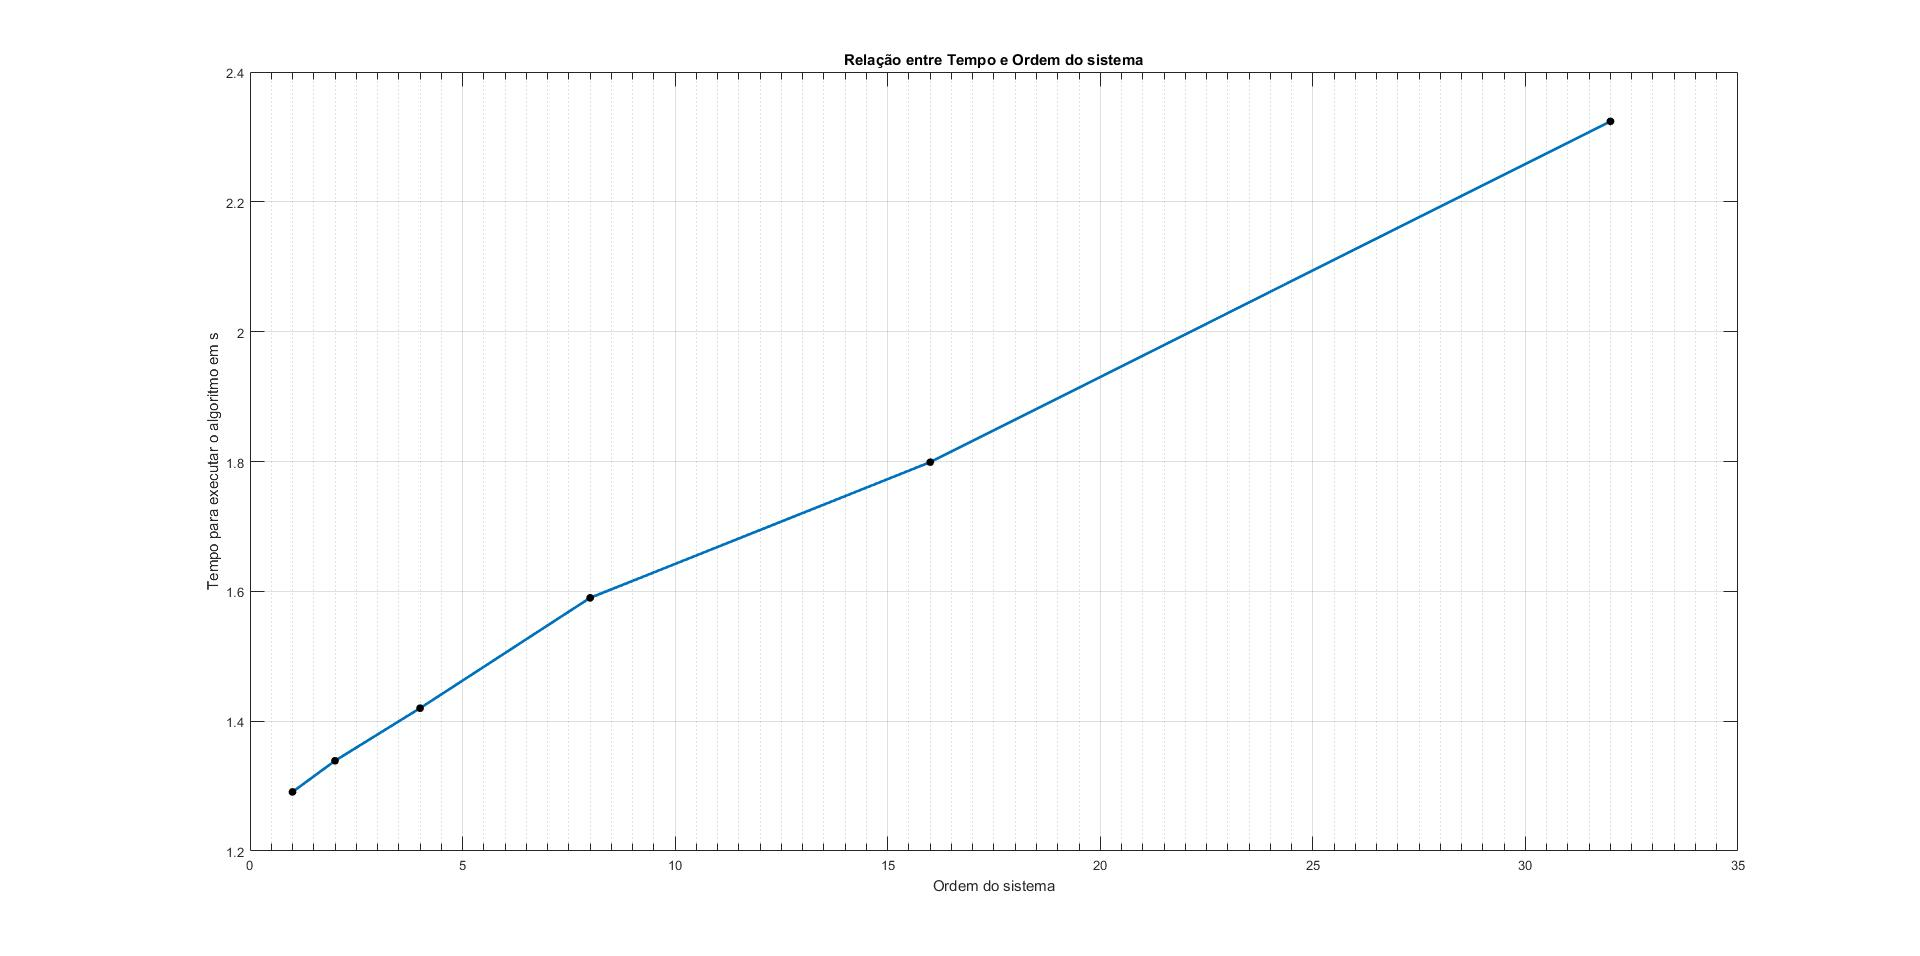
\includegraphics[width=1\linewidth]{figuras/TempoxOrdem.jpg}
	\caption{Relação entre tempo de processamento e a ordem do sistema}
	\label{fig:Tempo}
\end{figure}

A otimização do modelo para trabalhar somente no domínio da frequência e a implementação de um algoritmo em tempo real em um chip DSP podem ser uma solução para a implementação deste trabalho em um protótipo funcional. Além disso, a utilização de redes neurais aparenta ser uma solução para a criação de um modelo fiel a modelagem de sistemas não lineares, podendo desenvolver aplicações operando em tempo real com baixa latência. Arquiteturas implementadas com redes neurais podem ser treinadas com um conjunto de dados que fornece a resposta frequencial do amplificador utilizado como molde.